% =============================================================================
% HELD BACK from the thesis on 7 Oct 2026: the author judged the box-office analysis
% not relevant to the thesis. Not part of the Overleaf build. The analysis itself
% stays in the repository (results/box_office*.json, log sections 20 and 22).
% =============================================================================

% ---- was Section "Box Office (exploratory)" in chapter/3_evaluation.tex ----
% =============================================================================
\section{Box Office (exploratory)}
\label{sec:eval_boxoffice}

Whether commercial success relates to the soundtrack, or to how well its genre can be
recognised, is examined here as an exploratory side question.

The question is answered on the Blockbuster dataset, which suits it better than Eerola:
its 110 films were all released between 2014 and 2019, so their grosses are comparable
without an inflation adjustment, and a worldwide gross could be obtained for every one of
them from a single source, Box Office Mojo, after matching each film to its IMDb
identifier. A production budget was available for 84 of the films. Gross is skewed
(from USD 9 million to 2.8 billion), so every analysis uses its logarithm, and every
correlation is reported as Spearman's $\rho$ with a permutation $p$-value; within each
family of tests the $p$-values are corrected for multiple testing with the
Benjamini--Hochberg procedure. Pearson correlations on the logarithm and Kendall's $\tau$
were computed as well and lead to the same conclusions. Since Blockbuster has no
ratings, the emotions are those the Eerola-trained model predicts for each cue, averaged
over the film. The analysis is exploratory, and none of it can be read causally.

\paragraph{Is a higher-grossing film easier to classify?} No. For every route (emotion,
direct VGGish, the PCA-8 control and the full MIR set) and in both settings, in-domain
and zero-shot (MIR in-domain only), the per-film quality of the genre prediction was
correlated with gross under six per-film metrics: $F_1$, Jaccard index, Hamming
accuracy, exact match, label-ranking average precision and the probability margin
between a film's true and false genres. Of these 42 correlations, the largest in size is
$\rho=+0.243$ (PCA-8, in-domain Jaccard index), and none survives the correction for multiple
testing (smallest corrected $p=0.163$). The nominally significant ones do not form a
pattern. They occur for the direct and control routes in-domain but not for the emotion
route, and for the emotion route in the zero-shot setting only. How well a soundtrack
reveals its film's genre is unrelated to how much the film earned.

\paragraph{Do the soundtrack's emotions track gross?} Taken at face value they do, and
strongly (Figure~\ref{fig:box_office_blockbuster}). Higher-grossing films have angrier
($\rho=+0.427$), tenser ($+0.358$), more fearful ($+0.299$) and more energetic ($+0.227$)
scores, and less tender ($-0.366$), less positive in valence ($-0.317$) and less happy
($-0.255$) ones; all of these survive the correction. Their emotional range is also
wider. The spread of predicted anger and energy between a film's cues correlates with
gross at $+0.451$ and $+0.430$, and the number of cues at $+0.572$. Controlling for the
year of release does not change these results, but controlling for the budget removes
all the emotion correlations (only the number of cues keeps a weaker partial correlation,
$+0.225$): on the 84 films with a budget, every emotion's partial correlation with
gross lies between $-0.11$ and $+0.08$. Budget and gross are themselves strongly related
($\rho=+0.781$), and the genres that are expensive to make are the ones with the
angriest scores. Action films earn a median of USD 475 million against 129 million for
the rest, Sci-Fi films 615 against 159 million (both $p<0.001$), while Drama and Comedy
films earn less.

\begin{figure}[t]
  \centering
  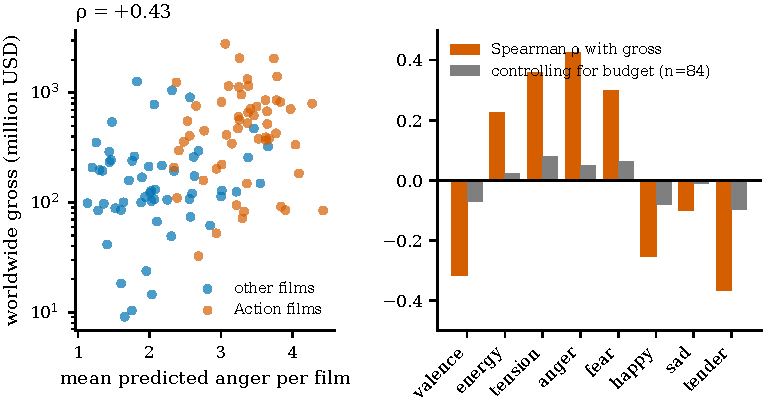
\includegraphics[width=\textwidth]{figures/box_office_blockbuster.pdf}
  \caption{Box office on the 110 Blockbuster films: gross against predicted anger, and emotion correlations with and without the budget.}
  \label{fig:box_office_blockbuster}
\end{figure}

The left panel of Figure~\ref{fig:box_office_blockbuster} plots worldwide gross (log
scale) against the mean predicted anger of a film's cues, with Action films highlighted.
The right panel gives the Spearman correlation of each predicted emotion with log gross,
as measured (orange) and after controlling for the production budget on the 84 films that
have one (grey).

\paragraph{Can gross be predicted from the soundtrack?} The single correlations above test
one feature at a time. As a multivariate check, a cross-validated ridge regression
($10\times5$ folds) predicted log gross from each representation. The soundtrack does
carry information about gross. The eleven emotion features explain $R^2=0.284$ of its
variance out of fold, the VGGish embedding $0.348$ and the MIR descriptors $0.214$, all
far above a permutation null. However, the six genre labels alone explain $0.253$, and
the budget alone explains $0.491$ on the 84 films that have one. On those films, the
emotions explain $0.118$, and adding them to the budget does not improve on the budget
alone ($0.452$). Taken one by one, 20 of the 139 non-constant MIR descriptors correlate
with gross after the correction, most of them timbral (MFCC means, spectral crest) or
rhythmic (pulse clarity).

The consistent reading is that a blockbuster's music reflects the scale and kind of
production rather than its success as such. Expensive action and science-fiction films
are scored with tense, angry, energetic music, use more of it, and earn more. Once the
budget is known, the soundtrack adds nothing to the prediction of gross. This agrees
with the check on Eerola described next.

\paragraph{The earlier check on Eerola.} An earlier and smaller check was made on the
Eerola films. A gross figure in US dollars could be matched by IMDb identifier for 37 of
them, and three readings of the question were tested with Spearman correlations and
permutation $p$-values. Classification quality does not relate to gross: the per-film
$F_1$ of the pipeline correlates with the logarithm of the gross at only $\rho=+0.197$
($p=0.246$). Genre does relate to it. Action films gross far more than the others
(median about USD 267 million against 44 million, Mann--Whitney $p=0.004$), and the
three Biography films far less ($p=0.045$, a result that rests on three films). Of the
eight emotions only anger correlates with gross at $p<0.05$ ($\rho=+0.335$, $p=0.043$),
and this is explained by genre: controlling for Action lowers it to $+0.191$, and within
the 28 non-Action films it is $+0.249$ ($p=0.196$). One nominal hit in eight tests is in
any case what chance often produces. The only robust relation is therefore the
unsurprising one that Action films are blockbusters, which concerns genre and not
anything the soundtrack model does. The check has clear limits: 37 films released between
1960 and 2006, worldwide grosses taken from two different sources (Wikidata and Box
Office Mojo), and no adjustment for inflation. Within those limits it agrees with the
Blockbuster analysis, in which gross relates to the kind of film and not to how well its
music reveals the genre.

% ---- was the paragraph "Box office." in the Limitations of chapter/discussion.tex ----
\paragraph{Box office.} The box-office analysis is exploratory and must not be read
causally. On the 110 Blockbuster films, how well a soundtrack reveals its genre is
unrelated to gross. The predicted emotions of the score, on the other hand, correlate
quite strongly with gross (the higher-grossing films have angrier, tenser and less tender
music) until the production budget is controlled for, at which point every correlation
disappears. The soundtrack therefore reflects the scale and kind of production and adds
nothing to predicting gross once the budget is known. The earlier check on 37 Eerola films
points the same way, since only genre relates to gross there. The analysis cannot separate
the many things a budget buys at once, such as a larger orchestra, more music, a franchise
or a marketing campaign. A larger sample would reduce its noise but not these confounds.
